% What is bio-informatics

\newcommand{\lf}{\tikz{\path[use as bounding box] (0,-.1) rectangle (0,.08);\path[draw=couleurtheme,very thick,|->] (0,0) -- (1.2,0);}}

\begin{frame}
  \frametitle{What is Bio-informatics?}

\begin{center}
\Large
  Confluence” of \tval{Biology} and \tval{Computer Science}
\end{center}

%\smallskip
\pause
\tval{Computer Science}: science of processing information

\pause
\medskip
\tval{Biology}: study of living organisms

\pause
\medskip
\begin{columns}
\begin{column}{.37\textwidth}

Many fields:
\begin{itemize}
  \item Sequencing
  \item \only<4>{Gene regulations}\only<5->{\tval{Gene regulations \lf}}
  \item Simulation
  \item Experiments
  \item …
\end{itemize}

~

~

\end{column}
\begin{column}{.55\textwidth}

\uncover<5->{
~

~

~

Approaches:
\begin{itemize}
  \item Differential equations
  \item \only<5>{Algebraic/qualitative}\only<6->{\tval{Algebraic/qualitative}}
  \item Hybrid
  \item Stochastic/probabilistic
  \item …
\end{itemize}
}

\end{column}
\end{columns}
\end{frame}



\begin{frame}
  \frametitle{Gene regulations}

\only<1>{\begin{center}
  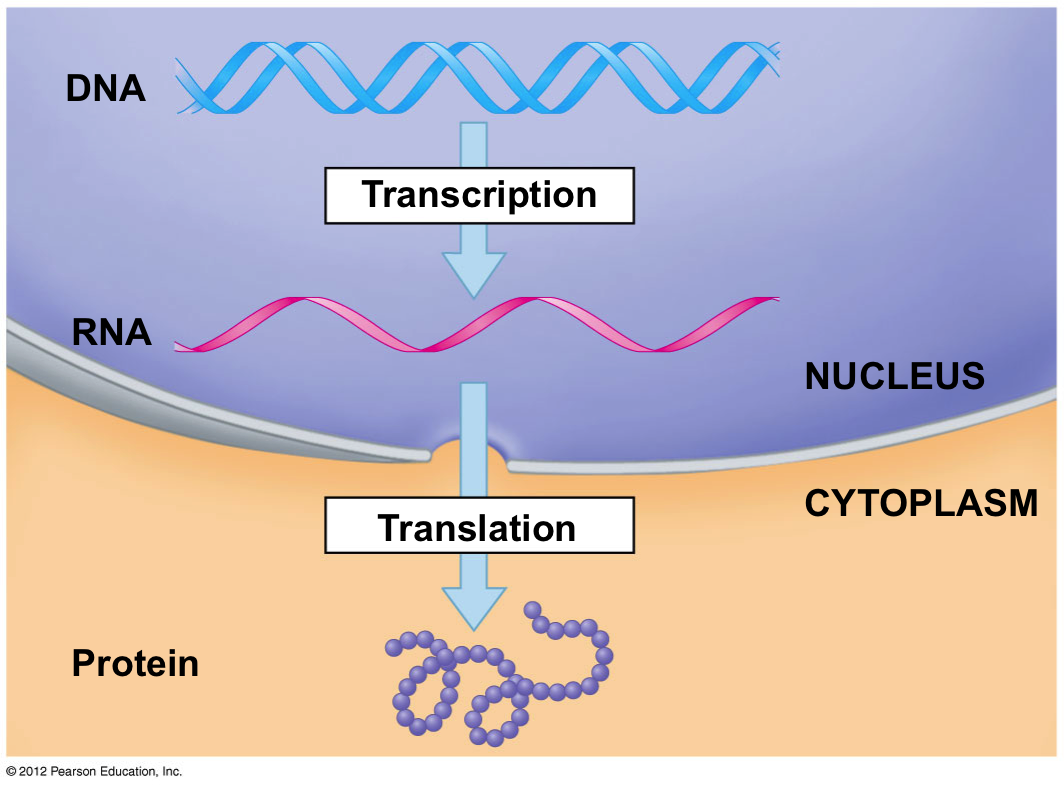
\includegraphics[width=.9\textwidth]{figs/protein.png}
\end{center}}
\only<2>{\begin{center}
  \scalebox{10}{
  \begin{tikzpicture}[adn]
    \node (a) {a};
  \end{tikzpicture}}
\end{center}}

\end{frame}



\newcommand{\noeud}[1]{\tikz[adn]{\path[use as bounding box] (-.25,-.1) rectangle (.25,.12);\node[inner sep=0] {#1};}}

\begin{frame}[c]
  \frametitle{Usual biological algebraic models}
  \framesubtitle{\tcite{\citedejong}}

\begin{center}
Modelling interacting genes/proteins:

%\bigskip

\scalebox{1.3}{
\begin{tikzpicture}[adn]
  \path[use as bounding box] (-0.7,-0.4) rectangle (2.5,2);
  \node[inner sep=0] (z) at (2,0.75) {z};
  \node[inner sep=0] (a) at (0,1.5) {a};
  \node[inner sep=0] (b) at (0,0) {b};
%  \path
%    node[elabel, above=-1em of a] {$\segm{0}{1}$}
%    node[elabel, below=-1em of b] {$\segm{0}{1}$}
%    node[elabel, below=-1em of z] {$\segm{0}{2}$};
  \path
    (a) edge[act,bend right=15] node[elabel,left] {$+$} (b)
    (b) edge[act,bend right=15] node[elabel,right] {$+$} (a)
    (b) edge[inh,loop left] node[elabel,left] {$-$} (b)
    (a) edge[inh] node[elabel,above] {$-$} (z)
    (b) edge[act] node[elabel,below] {$+$} (z);
\end{tikzpicture}}
\end{center}

\pause
\begin{columns}
\begin{column}{.6\textwidth}

Questions:
\begin{itemize}
  \item How does \noeud{z} \tval{behave}?
  \item Is it \tval{possible} to make \noeud{a} inactive?
  \item If I \tval{knock-out} \noeud{b}, what changes?
\end{itemize}

\end{column}
\end{columns}

\end{frame}
